% Options for packages loaded elsewhere
\PassOptionsToPackage{unicode}{hyperref}
\PassOptionsToPackage{hyphens}{url}
\PassOptionsToPackage{dvipsnames,svgnames,x11names}{xcolor}
%
\documentclass[
  letterpaper,
  DIV=11,
  numbers=noendperiod]{scrartcl}

\usepackage{amsmath,amssymb}
\usepackage{iftex}
\ifPDFTeX
  \usepackage[T1]{fontenc}
  \usepackage[utf8]{inputenc}
  \usepackage{textcomp} % provide euro and other symbols
\else % if luatex or xetex
  \usepackage{unicode-math}
  \defaultfontfeatures{Scale=MatchLowercase}
  \defaultfontfeatures[\rmfamily]{Ligatures=TeX,Scale=1}
\fi
\usepackage{lmodern}
\ifPDFTeX\else  
    % xetex/luatex font selection
\fi
% Use upquote if available, for straight quotes in verbatim environments
\IfFileExists{upquote.sty}{\usepackage{upquote}}{}
\IfFileExists{microtype.sty}{% use microtype if available
  \usepackage[]{microtype}
  \UseMicrotypeSet[protrusion]{basicmath} % disable protrusion for tt fonts
}{}
\makeatletter
\@ifundefined{KOMAClassName}{% if non-KOMA class
  \IfFileExists{parskip.sty}{%
    \usepackage{parskip}
  }{% else
    \setlength{\parindent}{0pt}
    \setlength{\parskip}{6pt plus 2pt minus 1pt}}
}{% if KOMA class
  \KOMAoptions{parskip=half}}
\makeatother
\usepackage{xcolor}
\setlength{\emergencystretch}{3em} % prevent overfull lines
\setcounter{secnumdepth}{-\maxdimen} % remove section numbering
% Make \paragraph and \subparagraph free-standing
\makeatletter
\ifx\paragraph\undefined\else
  \let\oldparagraph\paragraph
  \renewcommand{\paragraph}{
    \@ifstar
      \xxxParagraphStar
      \xxxParagraphNoStar
  }
  \newcommand{\xxxParagraphStar}[1]{\oldparagraph*{#1}\mbox{}}
  \newcommand{\xxxParagraphNoStar}[1]{\oldparagraph{#1}\mbox{}}
\fi
\ifx\subparagraph\undefined\else
  \let\oldsubparagraph\subparagraph
  \renewcommand{\subparagraph}{
    \@ifstar
      \xxxSubParagraphStar
      \xxxSubParagraphNoStar
  }
  \newcommand{\xxxSubParagraphStar}[1]{\oldsubparagraph*{#1}\mbox{}}
  \newcommand{\xxxSubParagraphNoStar}[1]{\oldsubparagraph{#1}\mbox{}}
\fi
\makeatother


\providecommand{\tightlist}{%
  \setlength{\itemsep}{0pt}\setlength{\parskip}{0pt}}\usepackage{longtable,booktabs,array}
\usepackage{calc} % for calculating minipage widths
% Correct order of tables after \paragraph or \subparagraph
\usepackage{etoolbox}
\makeatletter
\patchcmd\longtable{\par}{\if@noskipsec\mbox{}\fi\par}{}{}
\makeatother
% Allow footnotes in longtable head/foot
\IfFileExists{footnotehyper.sty}{\usepackage{footnotehyper}}{\usepackage{footnote}}
\makesavenoteenv{longtable}
\usepackage{graphicx}
\makeatletter
\newsavebox\pandoc@box
\newcommand*\pandocbounded[1]{% scales image to fit in text height/width
  \sbox\pandoc@box{#1}%
  \Gscale@div\@tempa{\textheight}{\dimexpr\ht\pandoc@box+\dp\pandoc@box\relax}%
  \Gscale@div\@tempb{\linewidth}{\wd\pandoc@box}%
  \ifdim\@tempb\p@<\@tempa\p@\let\@tempa\@tempb\fi% select the smaller of both
  \ifdim\@tempa\p@<\p@\scalebox{\@tempa}{\usebox\pandoc@box}%
  \else\usebox{\pandoc@box}%
  \fi%
}
% Set default figure placement to htbp
\def\fps@figure{htbp}
\makeatother

\KOMAoption{captions}{tableheading,figureheading}
\makeatletter
\@ifpackageloaded{caption}{}{\usepackage{caption}}
\AtBeginDocument{%
\ifdefined\contentsname
  \renewcommand*\contentsname{Table of contents}
\else
  \newcommand\contentsname{Table of contents}
\fi
\ifdefined\listfigurename
  \renewcommand*\listfigurename{List of Figures}
\else
  \newcommand\listfigurename{List of Figures}
\fi
\ifdefined\listtablename
  \renewcommand*\listtablename{List of Tables}
\else
  \newcommand\listtablename{List of Tables}
\fi
\ifdefined\figurename
  \renewcommand*\figurename{Figure}
\else
  \newcommand\figurename{Figure}
\fi
\ifdefined\tablename
  \renewcommand*\tablename{Table}
\else
  \newcommand\tablename{Table}
\fi
}
\@ifpackageloaded{float}{}{\usepackage{float}}
\floatstyle{ruled}
\@ifundefined{c@chapter}{\newfloat{codelisting}{h}{lop}}{\newfloat{codelisting}{h}{lop}[chapter]}
\floatname{codelisting}{Listing}
\newcommand*\listoflistings{\listof{codelisting}{List of Listings}}
\makeatother
\makeatletter
\makeatother
\makeatletter
\@ifpackageloaded{caption}{}{\usepackage{caption}}
\@ifpackageloaded{subcaption}{}{\usepackage{subcaption}}
\makeatother

\usepackage{bookmark}

\IfFileExists{xurl.sty}{\usepackage{xurl}}{} % add URL line breaks if available
\urlstyle{same} % disable monospaced font for URLs
\hypersetup{
  pdftitle={Global Renewable Energy Leaders in 2023},
  pdfauthor={Arisara Therdthianwong; Quanyu Qian; Dhruv Kaushal Gal},
  colorlinks=true,
  linkcolor={blue},
  filecolor={Maroon},
  citecolor={Blue},
  urlcolor={Blue},
  pdfcreator={LaTeX via pandoc}}


\title{Global Renewable Energy Leaders in 2023}
\author{Arisara Therdthianwong \and Quanyu Qian \and Dhruv Kaushal Gal}
\date{}

\begin{document}
\maketitle

\renewcommand*\contentsname{Table of Contents}
{
\hypersetup{linkcolor=}
\setcounter{tocdepth}{3}
\tableofcontents
}

\subsection{Executive summary}\label{executive-summary}

This report investigates the top 10 countries with the highest renewable
energy share in 2023 and global trends in energy transitions. It further
analyzes the sources of renewable energy in the leading country. The
analysis is conducted using reliable data from Our World in Data. Among
these countries, Norway stands out as a global leader with 72.09\% of
its primary energy coming from renewable sources. The findings offer
valuable insight to effectively implement national approaches that could
transform sustainable energy transitions worldwide.

\newpage

\subsection{Introduction}\label{introduction}

The global energy landscape has transformed rapidly in the last few
decades. Many countries are undergoing a major shift toward adopting
renewable sources such as hydropower, wind, and solar in response to the
challenges of climate change and resource sustainability. Renewable
energy now plays an important role as an alternative source that helps
to reduce reliance on fossil fuels and mitigate greenhouse gas
emissions.

Throughout the report, global renewable energy trends are identified,
with a focus on the top 10 countries with highest proportion of
renewable energy in total energy consumption in 2023. Norway leads the
way, with roughly 72\% of primary energy sourced from renewable. Sweden
and Brazil are also undergoing significant transitions, with 53.9\% and
50.3\% renewable shares, respectively.

A deeper analysis on Norway has been conducted to better understand how
a developed country manages its energy infrastructure achieving a high
level of renewable integration. Understanding these factors behind
Norway's performance can be beneficial for planning and improving
renewable energy policies and strategies that could be adapted to
different regional and national contexts. This analysis aims to provide
a useful insight that can guide future energy transitions globally.

\newpage

\section{Methodology}\label{methodology}

To identify the global leaders in renewable energy share, we used the
publicly available dataset from Our World in Data, which includes annual
records of renewable energy share by country from 1965 to 2023.

We filtered the dataset to focus exclusively on 2023 and excluded
aggregated regions (e.g., World, Europe, Asia), allowing us to rank
individual countries by their share of primary energy from renewables.

Table~\ref{tbl-table-top10} lists the top 10 countries with the highest
renewable energy share in 2023, and Figure~\ref{fig-top10-bar} presents
a bar chart for direct visual comparison.

To understand why Norway ranks highest globally, we analyzed its
national renewable energy composition using a second dataset on
electricity generation by source. We examined hydropower, wind, solar,
and bioenergy to assess their respective contributions. This breakdown
(Table~\ref{tbl-table-norway-2023} and Figure~\ref{fig-norway-sources})
shows Norway's strong dependence on hydropower, which contributes over
90\% of its renewable electricity output.

To complement Norway's national breakdown, we further compared its
hydropower generation to other global producers. Although Norway relies
heavily on hydropower as a share of its energy mix,
Figure~\ref{fig-global-hydro} reveals that its total generation is also
globally significant---enabling a clearer comparison between scale and
proportion in renewable leadership.

\subsection{Top 10 Countries by Renewable Energy Share in
2023}\label{top-10-countries-by-renewable-energy-share-in-2023}

We filtered the dataset to include only the year 2023. The processed
data identifies the top 10 countries with the highest share of renewable
energy.

Table~\ref{tbl-table-top10} lists these countries;
Figure~\ref{fig-top10-bar} visualizes the comparison.

\begin{longtable}[]{@{}llrr@{}}

\caption{\label{tbl-table-top10}Top 10 Countries by Share of Renewable
Energy in 2023}

\tabularnewline

\toprule\noalign{}
Country & Code & Year & Renewables (\%) \\
\midrule\noalign{}
\endhead
\bottomrule\noalign{}
\endlastfoot
Norway & NOR & 2023 & 72.09110 \\
Sweden & SWE & 2023 & 53.89018 \\
Brazil & BRA & 2023 & 50.33141 \\
Denmark & DNK & 2023 & 42.73486 \\
New Zealand & NZL & 2023 & 42.26695 \\
Austria & AUT & 2023 & 40.08019 \\
Switzerland & CHE & 2023 & 38.32534 \\
Portugal & PRT & 2023 & 36.04341 \\
Finland & FIN & 2023 & 35.93626 \\
South and Central America (EI) & NA & 2023 & 35.39018 \\

\end{longtable}

\begin{figure}

\caption{\label{fig-top10-bar}Top 10 Countries by Renewable Share in
2023}

\centering{

\pandocbounded{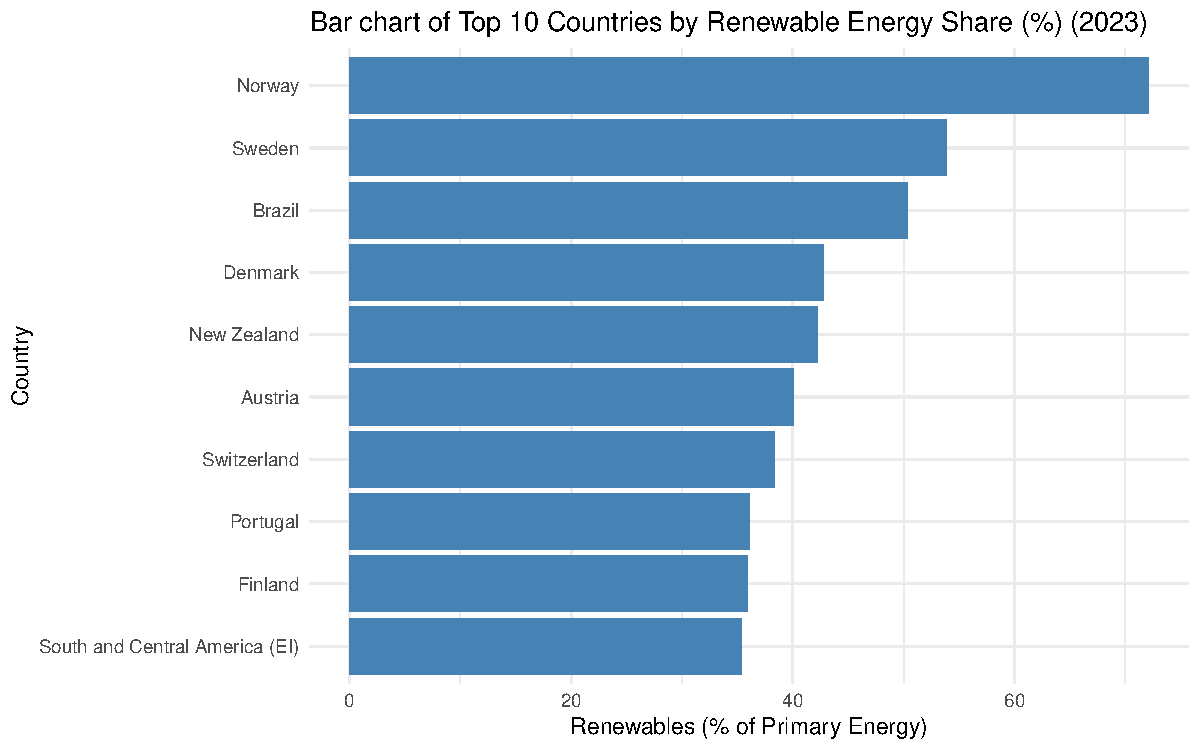
\includegraphics[keepaspectratio]{Assignment3_files/figure-pdf/fig-top10-bar-1.pdf}}

}

\end{figure}%

\subsection{Which country leads in renewable energy share in
2023?}\label{which-country-leads-in-renewable-energy-share-in-2023}

Norway ranked first in 2023 by renewable energy share.

To explore why Norway ranked first, we filtered its national records to
analyze its renewable energy sources.

\begin{longtable}[]{@{}lr@{}}

\caption{\label{tbl-table-norway-2023}Norway's Renewable Electricity
Generation by Source in 2023 (TWh)}

\tabularnewline

\toprule\noalign{}
Source & TWh \\
\midrule\noalign{}
\endhead
\bottomrule\noalign{}
\endlastfoot
wind & 14.96 \\
hydro & 135.96 \\
solar & 0.17 \\
Other renewables including bioenergy & 0.26 \\

\end{longtable}

\begin{figure}

\caption{\label{fig-norway-sources}Breakdown of Norway's Renewable
Energy Generation in 2023}

\centering{

\pandocbounded{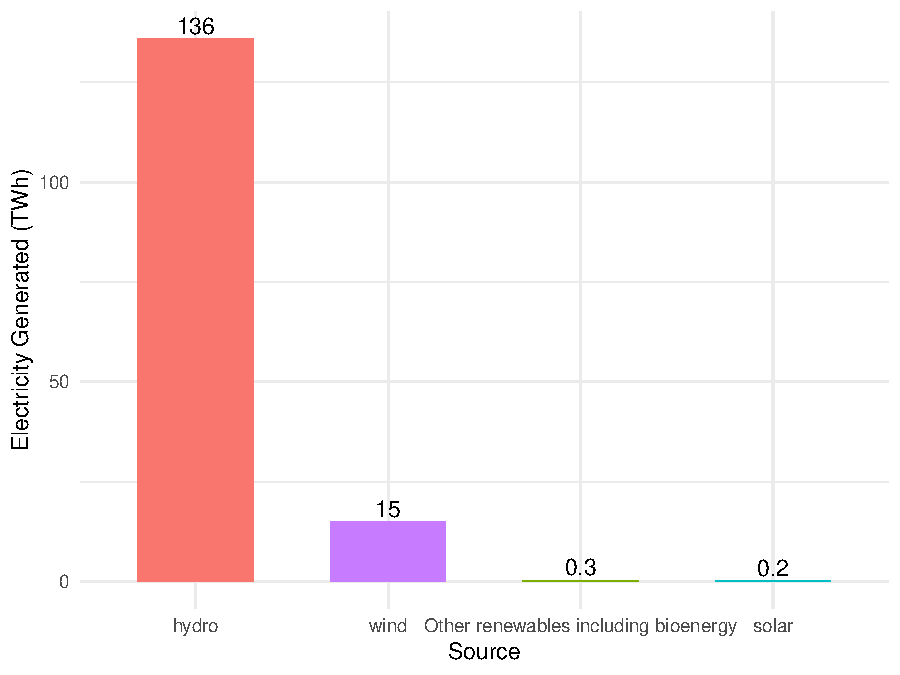
\includegraphics[keepaspectratio]{Assignment3_files/figure-pdf/fig-norway-sources-1.pdf}}

}

\end{figure}%

As shown in Figure~\ref{fig-norway-sources}, Norway's renewable
electricity in 2023 is dominated by hydropower, which accounts for
approximately 136 TWh, making up more than 90\% of its total renewable
output. In comparison, wind energy contributed around 15 TWh, which is
only about 10\% of the total. Both solar energy and other renewables
including bioenergy made negligible contributions, with values of 0.17
TWh and 0.26 TWh, respectively.

The limited output from wind and solar indicates that while Norway has
made some effort to diversify, its renewable success is not based on
technological breadth, but rather on natural geographic advantages.

This clear energy profile lays the foundation for further analysis in
the Results section, where we explore the historical, policy, and
environmental factors that have enabled Norway's exceptional performance
in renewable integration.

\subsection{Why Norway ranks highest globally in renewable energy
share?}\label{why-norway-ranks-highest-globally-in-renewable-energy-share}

To further explain why Norway ranks highest globally in renewable energy
share, we compare its energy source composition with that of other
top-performing countries.

\begin{figure}

\caption{\label{fig-global-hydro}Global Hydropower Generation (TWh) in
2023 by Country}

\centering{

\pandocbounded{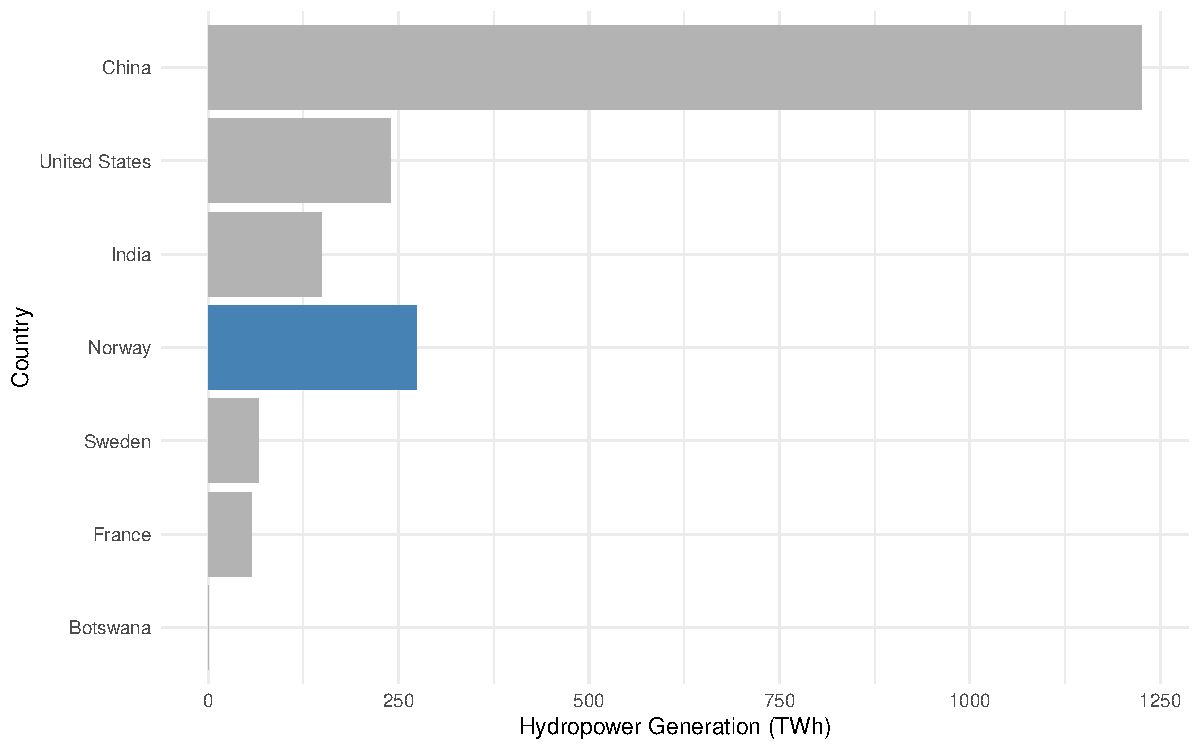
\includegraphics[keepaspectratio]{Assignment3_files/figure-pdf/fig-global-hydro-1.pdf}}

}

\end{figure}%

Figure~\ref{fig-global-hydro} compares total hydropower generation in
2023 across selected countries. While China leads with over 1,200 TWh,
Norway still ranks among the global top producers with approximately 270
TWh --- despite its relatively small population and geographic size.
This reinforces the idea that Norway's dominance in renewable energy
share is not just a percentage artifact, but supported by substantial
hydropower infrastructure and generation capacity. Norway's natural
topography has enabled it to produce a significant amount of clean
energy with low variability.




\end{document}
